\section{Theorien}

\subsection{FreeRTOS}

FreeRTOS ist ein leichtgewichtiges, quelloffenes \ac{RTOS}, das speziell für
Mikrocontroller und eingebettete Systeme entwickelt wurde. Es zeichnet sich
unter anderem durch deterministisches Verhalten mit Echtzeitgarantie sowie
Konfigurierbarkeit von Heap-Allokationen aus. Diese Eigenschaften machen es zu
einer geeigneten Wahl für mehrfädige Software, insbesondere wenn
Echtzeitanforderungen oder fein abgestimmte Kontrolle über Ressourcennutzung im
Vordergrund stehen.

\subsubsection{Features}

FreeRTOS unterscheidet sich von der Bare-Metal-Programmierung dadurch, dass es
einen umfangreichen Abstraktionslayer für den Nutzer bereitstellt. Diese
Abstraktionen ermöglichen es, komplexe (Echtzeit-)Operationen zu bewältigen,
ohne dass der Nutzer die benötigte Funktionalitäten selbst implementieren muss.
Beispiele hierfür sind unter anderem Timer mit konfigurierbarer Genauigkeit
(basierend auf den sogenannten Tick \cite{freertos_rtos_tick,
freertos_tick_resolution}), Queues, Semaphore sowie Mutexe.

Im Fokus dieser Arbeit stehen Queues und auch die sogenannte „Direct Task
Notifications“, die für den Datenaustausch verwendet werden. Ebenfalls relevant
sind Mutexe und „Trace Hooks“ für die darauffolgende Echtzeitanalyse. Diese
Komponenten werden im Folgenden detailliert erläutert.

\paragraph{Queues}

Queues sind eine Kernkomponente von FreeRTOS. Sie ermöglichen nicht nur eine
Interprozesskommunikation durch threadsicheren FIFO-Datenaustausch zwischen
Tasks, sondern dienen auch als Synchronisationsmechanismen: Die Semaphore und
Mutexe sind schlicht auf Queues aufgebaut \cite{freertos_semphr_incl}.

\paragraph{Semaphore und Mutexe} \label{sec:mutex}

Semaphore und Mutexe dienen zur Zugriffskoordinierung auf gemeinsame Ressourcen.
Im Vergleich zu Mutexen sind Semaphore aber besonders geeignet für die
Synchronisation beispielsweise zwischen Tasks oder Interrupts aufgrund ihrer
Einfachheit \cite{freertos_semphr_doc}. Sie sind nämlich
Synchronisationsmechanismen \textbf{ohne} Prioritätsvererbung -- ein Konzept,
bei dem eine niedriger priorisierte Task, die einen \textit{Mutex} hält,
temporär auf die Priorität der wartenden Task angehoben
wird~\cite{wikipedia_priority_inheritance}. Diese Funktionalität eignet sich
besonders gut für eine effiziente Zugriffskoordinierung auf gemeinsame
Ressourcen -- was mit Semaphoren nicht gewährleistet werden kann und folglich zu
Prioritätsinversion führen kann: Eine höher priorisierte Task wird blockiert,
während der Scheduler eine andere, niedriger priorisierte Task ausführt, die die
benötigte Ressource nicht besitzt -- und das so lange, bis die Task mit der
benötigten Ressource diese freigibt \cite{wikipedia_priority_inversion}.

Die folgenden Sequenzdiagramme zeigen den Vergleich zwischen Prioritätsinversion
bei Verwendung eines Semaphors und der Prioritätsvererbung bei einem Mutex,
dargestellt an drei Tasks mit unterschiedlichen Prioritätsstufen:

\begin{figure}[H]
    \centering
    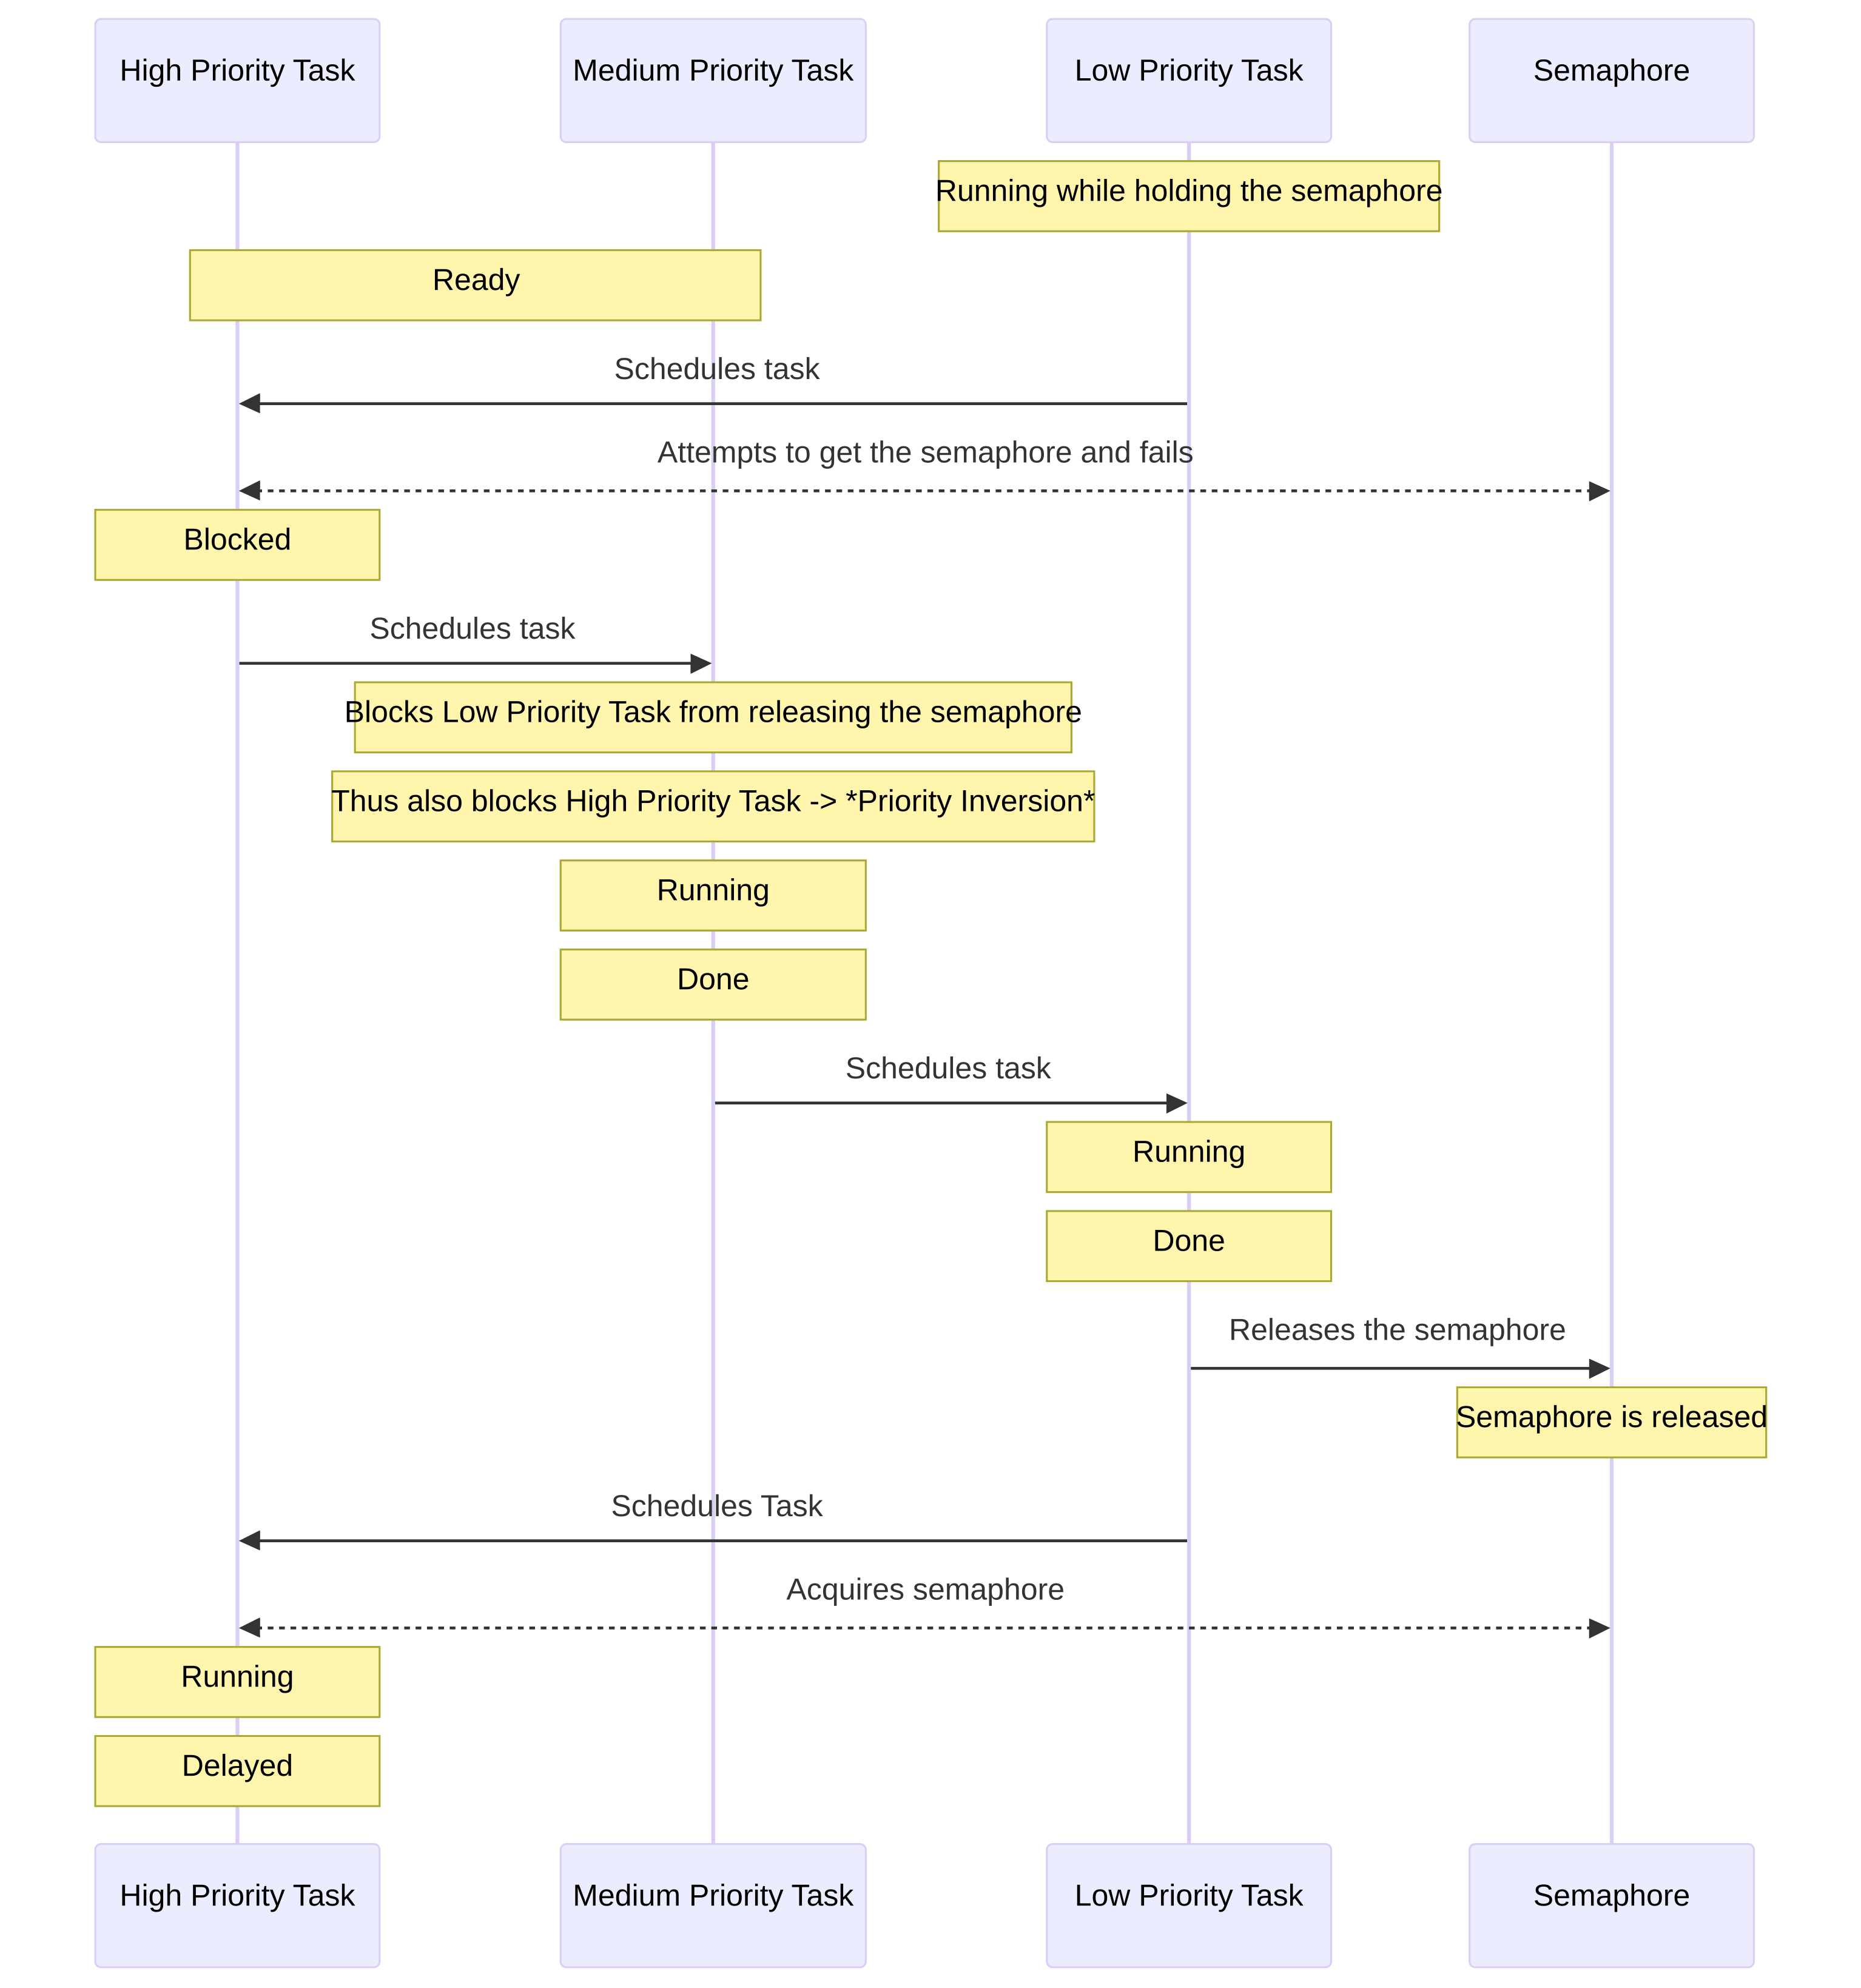
\includegraphics[width=1\textwidth]{assets/prio_inversion}
    \caption{Prioritätsinversion}
\end{figure}

\begin{figure}[H]
    \centering
    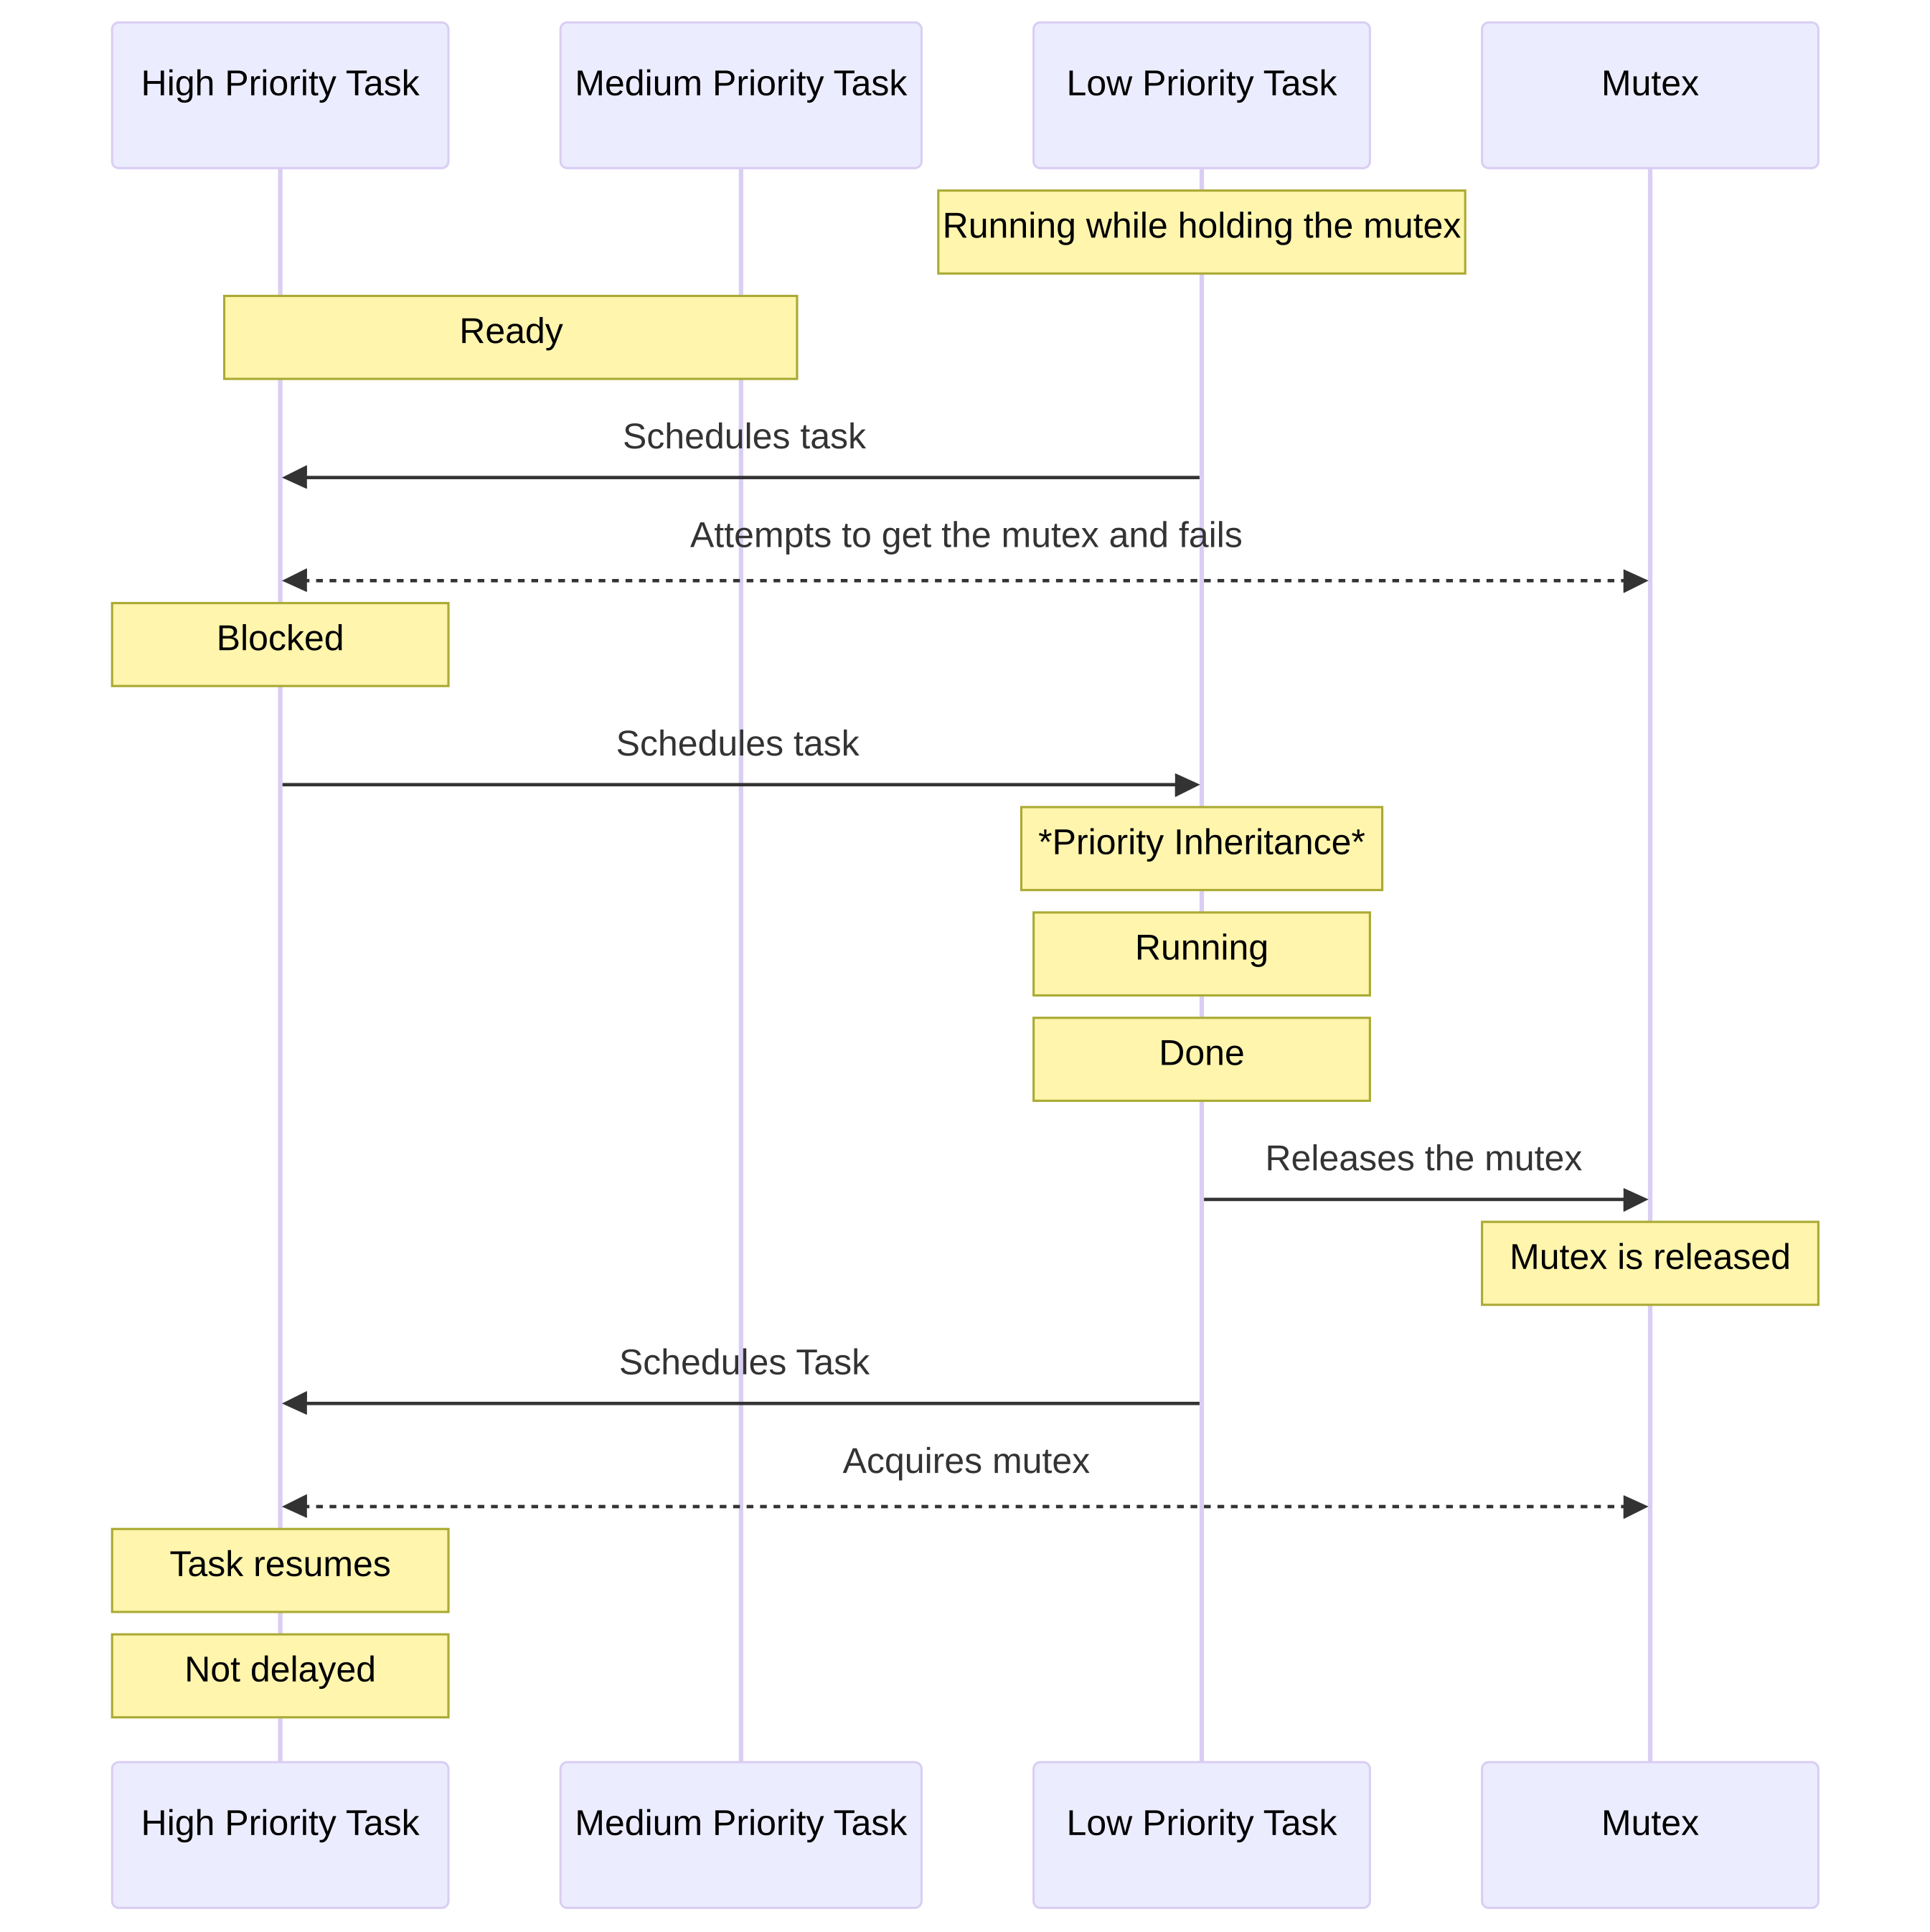
\includegraphics[width=1\textwidth]{assets/prio_inheritance}
    \caption{Prioritätsvererbung}
\end{figure}

\paragraph{Direct-Task-Notifications} \label{sec:direct_task_notification}

Direct-Task-Notifications sind ein effizienterer und ressourcenschonenderer
Mechanismus zur Task-Synchronisation \cite{freertos_task_notifications_desc}.
Insbesondere soll das Entblocken einer Task mittels Direct-Task-Notifications
bis zu 45\% schneller sein und weniger RAM benötigen
\cite{freertos_task_notifications_usage}. Im Gegensatz zu Semaphoren, die als
zusätzliche separate Objekte fungieren, koordinieren die Tasks miteinander
direkt durch einen internen Zählers \cite{freertos_tasks_c_308}. Analog zur
Verwendung von Semaphoren wird mittels Funktionen wie
\mintinline{c}|xTaskNotifyGive()| dieser Zähler
inkrementiert~\cite{freertos_tasks_c_4990}, während
\mintinline{c}|ulTaskNotifyTake()| ihn wieder
dekrementiert~\cite{freertos_tasks_c_4614}.

\paragraph{Trace Hooks} \label{sec:trace_hooks}

„Trace Hooks“ sind spezielle, von FreeRTOS bereitgestellte Makros. Sie
ermöglichen beispielsweise die Verfolgung oder Protokollierung von
Systemereignissen. Diese Makros werden direkt innerhalb von Interrupts beim
Scheduling aufgerufen und sollten stets vor der Einbindung von
\mintinline{text}|FreeRTOS.h| definiert werden \cite{freertos_rtos_trace_hooks}.

\subsection{Nutzung von Caches}

Caches sind schnelle Speicherkomponenten, die dazu dienen, Zugriffe auf häufig
verwendete Daten und Befehle zu beschleunigen und den Energieverbrauch zu
reduzieren \cite{ka001150}. In vielen modernen Mikrocontrollern, wie dem
Cortex-M7, ist der L1-Cache (Level 1 Cache -- typischerweise die kleinste aber
schnellste Cachekomponente) jeweils in einen Datencache (D-Cache) sowie einen
Instruktionscache (I-Cache) unterteilt \cite[S. 6]{an4667}. Da Zugriffe auf den
Flash-Speicher deutlich langsamer sind und mehrere Taktzyklen
benötigen~\cite{stm32_memory_sections}, ermöglichen L1-Caches
Zero-Wait-State-Zugriffe~\cite[S. 6]{an4667}: der Prozessor kann ohne
zusätzliche Wartezyklen auf Daten zugreifen \cite{waitstate_wiki}.

Der L1-Cache kann nur mit der \ac{AXI}-Busschnittstelle genutzt werden~\cite[S.
4]{an4839}. Hierzu zählen unter anderem der Flash, der \ac{SRAM} sowie die
Peripheriebusse, die alle über den \ac{AHB}-Bus an den AXI angebunden sind
(\ref{fig:m7_sys_arch}).

\begin{figure}[htb]
    \centering
    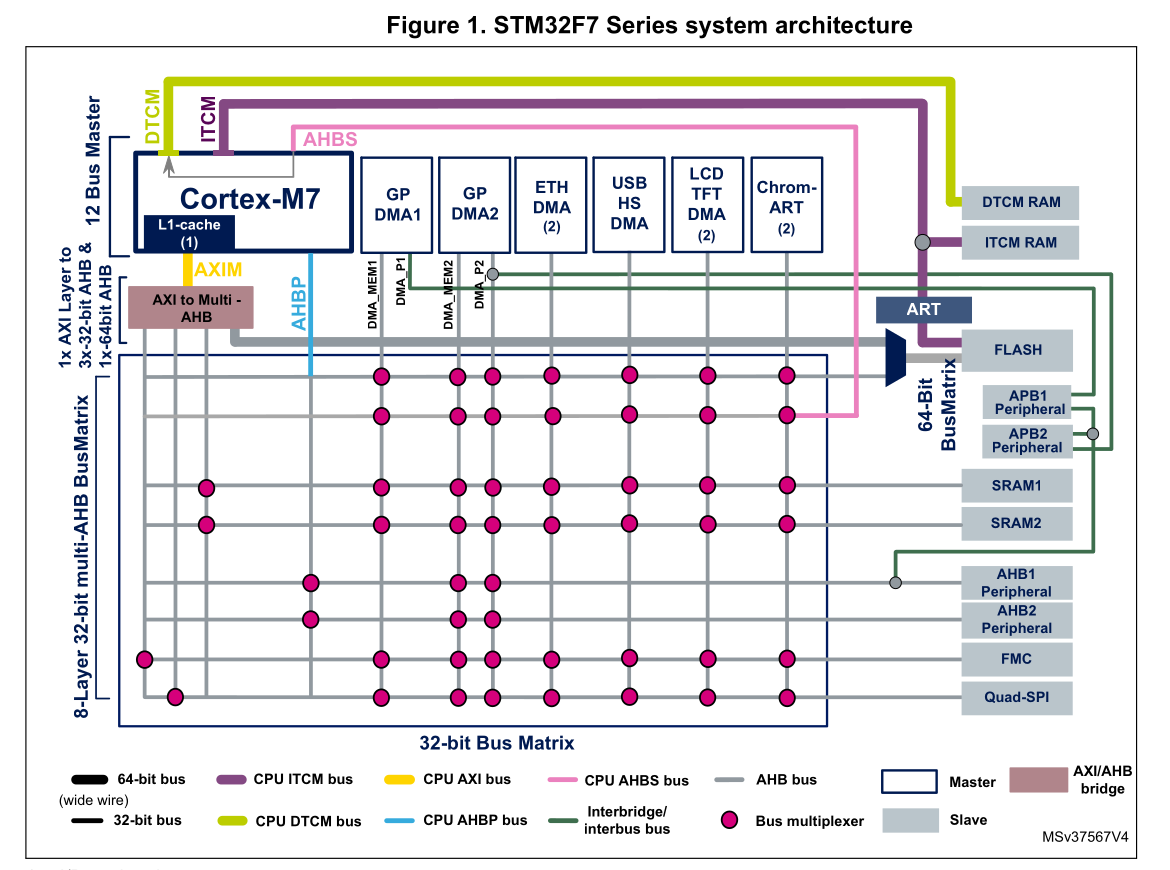
\includegraphics[width=1\textwidth]{assets/m7_system_arch}
    \caption{STM32F7 Systemarchitektur \cite[S. 9]{an4667}}
    \label{fig:m7_sys_arch}
\end{figure}

Aus der Matrix wird außerdem deutlich, dass für den Speicher zwischen SRAM und
TCM-RAM unterschieden wird. Der \ac{TCM} verfügt jeweils für Instruktionen und
Daten über einen dedizierten Kanal zum Prozessor und ist \textit{nicht}
cachefähig, bietet aber als Besonderheit niedrigere und konsistente
Zugriffszeiten als SRAM. Dies macht sie besonders geeignet für zeitkritische
Routinen wie Interrupt-Handler oder kritische Echtzeitaufgaben.
(\cite{arm_den0042})

Im Rahmen dieser Bachelorarbeit wird der TCM nicht genutzt und daher nicht
weiter betrachtet.

Zusammenfassend lässt sich sagen, dass jeder normale, nicht gemeinsam genutzte
(non-shared) Speicherbereich gecacht werden kann, sofern er über den AXI-Bus
zugänglich ist \cite[S. 4]{an4839}~\cite[S. 7]{an4667}.

\begin{figure}[htb]
    \centering
    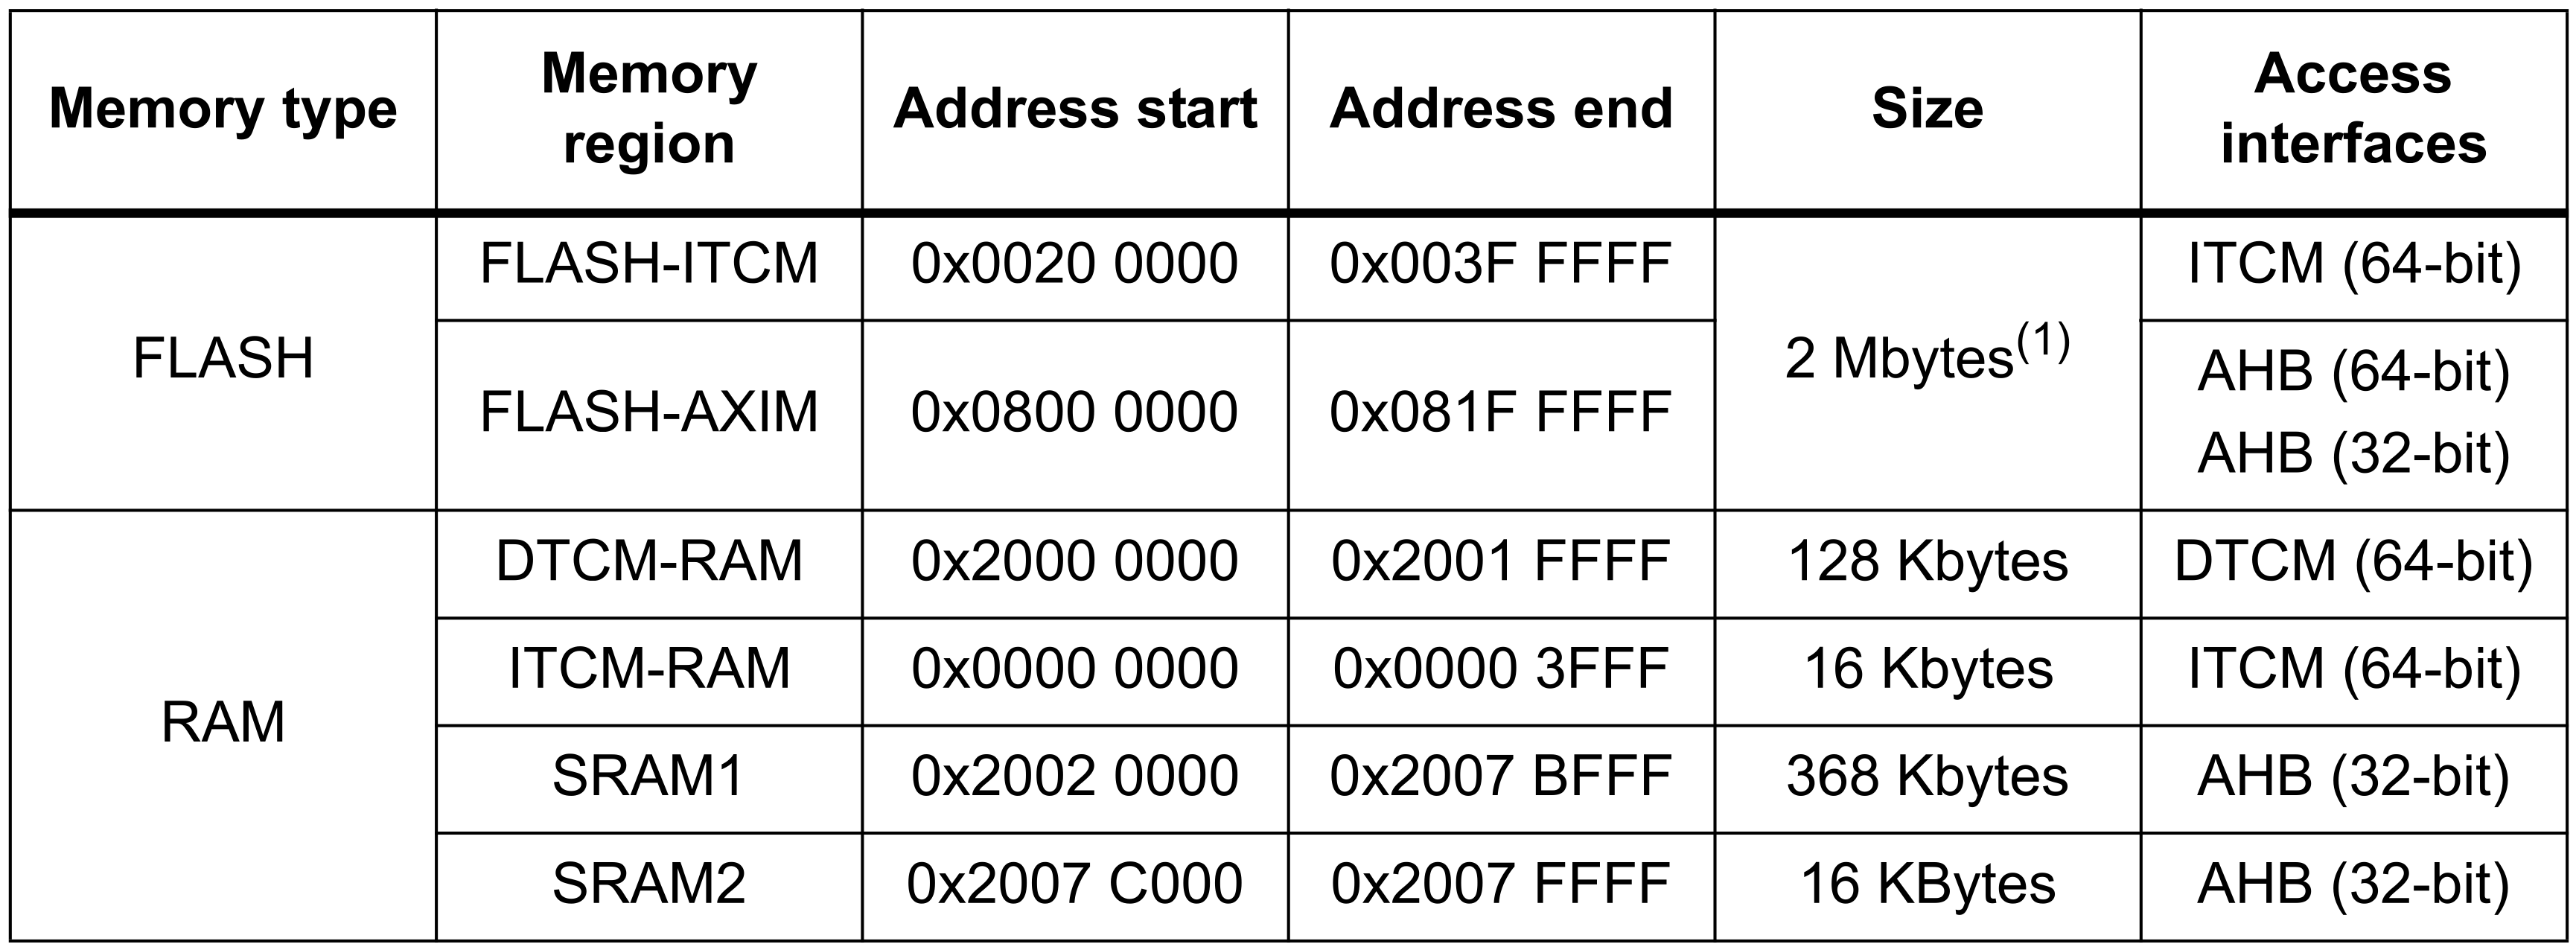
\includegraphics[width=1\textwidth]{assets/internal_mem_table}
    \caption{STM32F7 Speicheradressen \cite[S. 14]{an4667}}
    \label{fig:internal_mem_table}
\end{figure}

Aus der Tabelle für den internen Speicher wird deutlich, dass der Flash ab der
Adresse $0x0800 0000$ über der AXI-Bus angesprochen wird
(\ref{fig:internal_mem_table}). Diese Adresse ist auch im Linker-Skript
standardmäßig für den Flash festgelegt. Daher kann der Instruktionscache über
den AXI-Bus für den Flash genutzt werden, sofern der Boot-Pin sowie die
assoziierten \mintinline{text}|BOOT_ADDx| Registerkonfigurationen unverändert
bleiben und die Firmware an die Standardadresse geflasht wird \cite[S.
28]{stm32_datasheet}.

\begin{code}
\begin{minted}{c}
MEMORY
{
RAM (xrw)      : ORIGIN = 0x20000000, LENGTH = 512K
FLASH (rx)      : ORIGIN = 0x8000000, LENGTH = 2048K
}
\end{minted}
    \captionof{listing}{Definition Speicherbereich im Linker-Script für STM32F7}
\end{code}

Um Caches zu nutzen, bietet die STM-\ac{HAL} dedizierte Funktionen als API an
\cite[S. 4]{an4839}:

\begin{code}
\begin{minted}{c}
void SCB_EnableICache(void)
void SCB_EnableDCache(void)
void SCB_DisableICache(void)
void SCB_DisableDCache(void)
void SCB_InvalidateICache(void)
void SCB_InvalidateDCache(void)
void SCB_CleanDCache(void)
void SCB_CleanInvalidateDCache(void)
\end{minted}
    \captionof{listing}{Cache-Funktionen}
\end{code}

\subsubsection{Cache-Leerung}

Bei einer Cache-Leerung (cache clean) werden modifizierte Cache-Zeilen (dirty
cache lines), die vom Prozessor während der Programmausführung aktualisiert
wurden, zurück in den Hauptspeicher geschrieben \cite[S. 4]{an4839}. Dieser
Vorgang wird gelegentlich auch als „flush” bezeichnet.

\subsubsection{Cache-Invalidierung}

Eine Cache-Invalidierung markiert hingegen den Cache als ungültig, sodass bei
dem nachfolgenden Zugriff auf die assoziierten Daten diese zwingend erneut aus
dem Hauptspeicher geladen und der Cache entsprechend aktualisiert werden.

\subsubsection{Cache-Leerung bei DMA} \label{sec:cache_clean}

Allerdings kann bei der Nutzung von Caches für Speicherbereiche, die mit dem
DMA-Controller geteilt werden, ein Cache-Kohärenzproblem (Cache Coherency)
auftreten, da der Prozessor in diesem Fall nicht mehr der einzige Master ist,
der auf diese Speicherbereiche zugreift.

Damit der DMA-Controller stets auf korrekte Daten zugreifen kann, ist eine
manuelle Cache-Leerung \textit{nach} jedem Schreibvorgang von Seiten der CPU
erforderlich \cite[S. 6]{an4839}. Ohne diesen Schritt würden die Änderungen
nicht im SRAM widergespiegelt, und der DMA-Controller würde weiterhin
veraltete/ungültige Daten verwenden.

\subsubsection{Cache-Invalidierung bei DMA}

Bei Daten, die aus einem Speicherbereich gelesen werden, der auch vom
DMA-Controller modifiziert werden kann, ist \textit{vor} jedem Lesevorgang eine
Cache-Invalidierung notwendig \cite{embeddedexpert_cache}. Da der DMA-Controller
asynchron und unabhängig von der CPU schreiben kann, sind gecachten Daten
potenziell veraltet/ungültig, und müssen stets manuell aktualisiert werden.

\subsection{Methode zur Echtzeitanalyse} \label{sec:dwt}

Für die Echtzeitanalyse der Steuerungssoftware wird eine Methode benötigt, die
beliebige Softwareabschnitte flexibel, threadsicher und präzise vermessen kann.
Da es sich um eine mehrfädige Anwendung handelt, muss gewährleistet sein, dass
die Messungen trotz preemptivem Scheduling, parallel auftretenden Interrupts
sowie Compiler-Optimierung zyklengenau durchgeführt werden. Die Lösung muss
insbesondere garantieren, dass keine Race Conditions durch Kontextwechsel
entstehen und die Zeitmessung selbst keinen nennenswerten Overhead verursacht.

Daher bietet sich die \ac{DWT} als geeignete Lösung zur Protokollierung von
Zeiten an~\cite{ARM_KA001499}. Die DWT ist eine in vielen Prozessoren
standardmäßig eingebaute Debug-Einheit, die unter anderem das Profiling mittels
verschiedener Zähler unterstützen \cite{ARMv7_ref_man_dwt_profiling}. Ein für
diese Arbeit zentraler Baustein ist der Zyklenzähler \mintinline{c}|DWT_CYCCNT|,
der bei jedem CPU-Takt inkrementiert wird, solange sich der Prozessor nicht im
Debug-Zustand befindet \cite{ARMv7_ref_man_dwt_cycle}. Wie der Name bereits
vermuten lässt, ermöglicht die DWT die Protokollierung mit zyklengenauer
Präzision unter normaler Operation \cite{ARMv7_ref_man_dwt_profiling}.

\subsubsection{Beispiel: Segger SystemView}

Ein Beispiel hierfür ist Segger SystemView, ein Echtzeitanalyse-Tool, das die
DWT nutzt, um Live-Code-Profiling auf eingebetteten Systemen durchzuführen
\cite{SEGGER_SystemView}.

Das Segger SystemView nutzt den DWT-Zyklenzähler, indem die Funktion \linebreak
\mintinline{c}|SEGGER_SYSVIEW_GET_TIMESTAMP()| für Cortex-M3/4/7-Prozessoren
einfach die hardkodierte Registeradresse des Zyklenzählers zurückgibt \cite[S.
65]{Segger_SystemView_manual}\cite{Arm_DWT_Programmers_Model}, anstatt die
interne Funktion \mintinline{c}|SEGGER_SYSVIEW_X_GetTimestamp()| aufzurufen.
